\documentclass[11pt,a4paper]{article}
\usepackage{amsmath, amssymb, amsthm}
\usepackage{geometry}
\usepackage{graphicx}
\usepackage{url}
\usepackage{hyperref}
\usepackage[dvipsnames]{xcolor}
\usepackage{mylistings}
\usepackage[font=small,skip=4pt]{caption}
\usepackage{chngcntr,tocloft}

\counterwithin*{figure}{section}
\counterwithin*{figure}{subsection}
\counterwithin*{figure}{subsubsection}

\addtolength{\cftfignumwidth}{2em}


\renewcommand{\thefigure}{%
  \ifnum\value{subsection}=0
    \thesection.\arabic{figure}%
  \else
    \ifnum\value{subsubsection}=0
      \thesubsection.\arabic{figure}%
    \else
      \thesubsubsection.\arabic{figure}%
    \fi
  \fi
}

\renewcommand{\lstlistingname}{Algorithm}

\definecolor{codegreen}{rgb}{0,0.6,0}
\definecolor{codegray}{rgb}{0.5,0.5,0.5}
\definecolor{codepurple}{rgb}{0.58,0,0.82}
\definecolor{backcolour}{rgb}{1,1,1}

\lstdefinestyle{mystyle}{
    backgroundcolor=\color{backcolour},   
    commentstyle=\color{codegreen},
    keywordstyle=\color{magenta},
    numberstyle=\tiny\color{codegray},
    stringstyle=\color{codepurple},
    basicstyle=\ttfamily\footnotesize,
    breakatwhitespace=false,         
    breaklines=true,                 
    captionpos=b,                    
    keepspaces=true,                 
    numbers=left,                    
    numbersep=5pt,                  
    showspaces=false,                
    showstringspaces=false,
    showtabs=false,                  
    tabsize=2,
    frame=tb,
    framexleftmargin=5mm,
    xleftmargin=5mm,
    framexrightmargin=5mm,
    xrightmargin=5mm,
    rulecolor=\color{black},
    upquote=true,
    aboveskip=3mm,
    belowskip=3mm,
    captionpos=b
}

\lstset{style=mystyle}

\parindent 0pt

\geometry{margin=1in}
\renewcommand{\contentsname}{Contents}

\renewcommand{\baselinestretch}{1.25}
\renewcommand{\contentsname}{Contents}

\usepackage{hyperref}
\hypersetup{
    colorlinks,
    citecolor=blue,
    filecolor=blue,
    linkcolor=blue,
    urlcolor=blue
}

\usepackage{enumitem}

\usepackage{cleveref}
\crefname{section}{\S}{\S\S}
\Crefname{section}{\S}{\S\S}
\crefname{subsection}{\S}{\S\S}
\Crefname{subsection}{\S}{\S\S}

\begin{document}

% Titlepage
\newpage
\begin{titlepage}
    \vspace*{\fill} % add vertical space before content
    \centering
    \huge{\textbf{CS477 -- Computer Vision}} \\
    \huge{Assignment 1} \\ [0.75cm]
    \begin{figure}[ht!]
        \centering
        
\includegraphics[width=0.5\textwidth]{figs/nust.pdf}
    \end{figure}
    \vspace {0.75cm}
    \Large{By} \\
    \Large{\textbf{Muhammad Umer}\quad(CMS -- 345834)} \\
    \Large{\textbf{Muhammad Ahmed Mohsin}\quad(CMS -- 333060)} \\
    \Large{\textbf{Muhammad Saad}\quad(CMS -- 333414)} \\ [0.75cm]
    \Large{Instructor} \\
    \Large{\textbf{Dr. Mohsin Kamal}} \\[0.75cm]
    \Large{School of Electrical Engineering and Computer Science (SEECS) \\
        National University of Sciences and Technology (NUST) \\
        Islamabad, Pakistan} \\ [0.75 cm]
    \Large{\today}
    \vspace*{\fill} % add vertical space after content
\end{titlepage}

\tableofcontents

\newpage
\setcounter{page}{1}
\section{Introduction}

In this assignment, we delve into several fundamental image processing tasks, each aimed at demonstrating different aspects of image manipulation and analysis. The primary objective of this assignment is to develop a comprehensive understanding of various image processing techniques and their applications.

\subsection*{Deliverables}
\begin{enumerate}
    \item \textbf{Filtering Techniques:}
          \textit{\\Take any image and perform Gaussian filtering, box filtering and median filtering. Also provide comments on the results.}

    \item \textbf{Edge Detection:}
          \textit{\\Take any image and detect edges by using Sobel and Prewitt Kernel. Comment on both results.}

    \item \textbf{Histogram Representation:}
          \textit{\\Take any image and plot its histogram representation.}

    \item \textbf{Gray and Binary Representation:}
          \textit{\\Take a colored image and provide its gray and binary representation.}

    \item \textbf{Corner Detection:}
          \textit{\\Take any image and detect the corners by employing Harris corner detection.}
\end{enumerate}

\subsection*{Author Contributions}
Mention each author's contribution at the end of each question (Mandatory).
\begin{itemize}[itemsep=-1ex, topsep=0pt, leftmargin=1em]
    \color{RoyalBlue}\item \textbf{Author 1:} \color{black}{--}
          \color{RoyalBlue}\item \textbf{Author 2:} \color{black}{--}
          \color{RoyalBlue}\item \textbf{Author 3:} \color{black}{--}
\end{itemize}

\subsection*{Grading Scheme}
\textbf{\begin{itemize}[itemsep=-1ex, topsep=0pt, leftmargin=1em]
        \color{Maroon}
        \item Q1: 10 Marks
        \item Q2: 10 Marks
        \item Q3: 10 Marks
        \item Q4: 10 Marks
        \item Q5: 10 Marks
        \item Total: 50 marks
    \end{itemize}}

\subsection*{Copying}
Copying is highly discouraged and it will lead to a significant loss  (90-95 \%) of marks.

\textit{*Copying includes using sentences, variables, code, formats from others. Discussion is appreciated, but attempt the tasks on your own (which would make it look original).}

\newpage
\section{Task 1 -- Filtering Techniques}

\begin{lstlisting}[language=iPython, title=Python Code for Filtering Techniques]
    import cv2
    import numpy as np
    
    def get_gaussian_kernel(size, sigma=-1):
        """
        Generates a Gaussian kernel of the specified size and sigma.
    
        If sigma = -1, then sigma is automatically calculated
        as (size - 1) / 6.0, as per the OpenCV documentation.
        """
        if sigma < 0:
            sigma = (size - 1) / 6.0
    
        # Generate a grid using the specified size
        axis = np.linspace(-(size - 1) / 2.0, (size - 1) / 2.0, size)
        x, y = np.meshgrid(axis, axis)
    
        # Create the kernel
        gaussian_kernel = np.exp(-0.5 * (x**2 + y**2) / sigma**2)
    
        return gaussian_kernel / np.sum(gaussian_kernel)
    
    # Read image
    img = cv2.imread("./lenna.png")
    
    # Define kernel size
    kernel_size = 7
    
    # Define kernels
    box_kernel = (1 / kernel_size**2) * np.ones((kernel_size, 
                                                kernel_size))
    gaussian_kernel = get_gaussian_kernel(kernel_size, 5)
    
    # Apply filters
    box_filtered = cv2.filter2D(img, -1, box_kernel)
    gaussian_filtered = cv2.filter2D(img, -1, gaussian_kernel)
    median_filtered = cv2.medianBlur(img, kernel_size)
    
    # Save images
    cv2.imwrite("report/figs/task1/box_filtered.png", box_filtered)
    cv2.imwrite("report/figs/task1/gaussian_filtered.png",
                gaussian_filtered)
    cv2.imwrite("report/figs/task1/median_filtered.png", median_filtered)
    
    # Show images
    cv2.imshow("Original", img)
    cv2.imshow("Box Filtered", box_filtered)
    cv2.imshow("Gaussian Filtered", gaussian_filtered)
    cv2.imshow("Median Filtered", median_filtered)
    
    cv2.waitKey(0)
    cv2.destroyAllWindows()
\end{lstlisting}

\subsection*{Author Contributions \& Comments}
\begin{itemize}[itemsep=-1ex, topsep=0pt, leftmargin=1em]
    \color{RoyalBlue}\item \textbf{Author 1:} \color{black}{--} Devised a pseudo-code for the filtering techniques. Also put forth a layout for showing and saving images.
          \color{RoyalBlue}\item \textbf{Author 2:} \color{black}{--} Implemented the Gaussian kernel function and the Gaussian filtering.
          \color{RoyalBlue}\item \textbf{Author 3:} \color{black}{--} Implemented the box kernel function and box filtering. Also implemented the median filtering.
    \item \textbf{Comments:} Given that the original image had realistic noise, the Gaussian filtered image was the least blurred while effectively suppressing noise. On the other hand, the median filter suppressed noise, but at the cost of losing edge clarity, as expected since the median filter is better suited for salt-and-pepper noise. Similarly, the box filter yielded a uniformly blurred image, losing information about edges.
\end{itemize}

% 4 subfigures, each with different caption
\subsubsection*{Results}
\begin{figure}[ht!]
    \centering
    \begin{minipage}{0.3\textwidth}
        \centering
        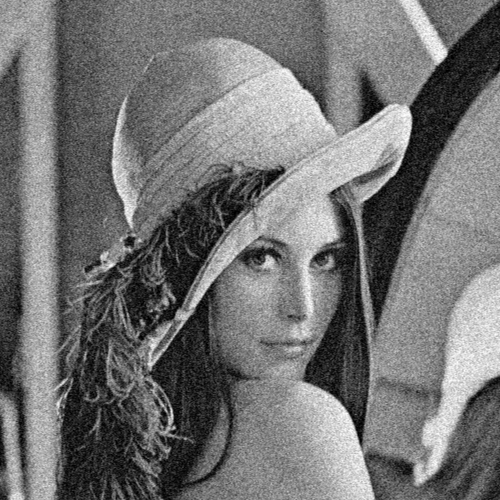
\includegraphics[width=\linewidth]{figs/lenna_noisy.png}
        \caption{Original (Noisy)}
    \end{minipage}
    \quad
    \begin{minipage}{0.3\textwidth}
        \centering
        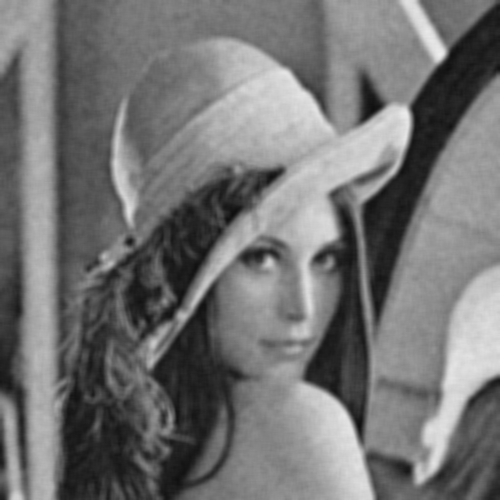
\includegraphics[width=\linewidth]{figs/task1/box_filtered.png}
        \caption{Box Filtered}
    \end{minipage}
    \vskip 4pt
    \begin{minipage}{0.3\textwidth}
        \centering
        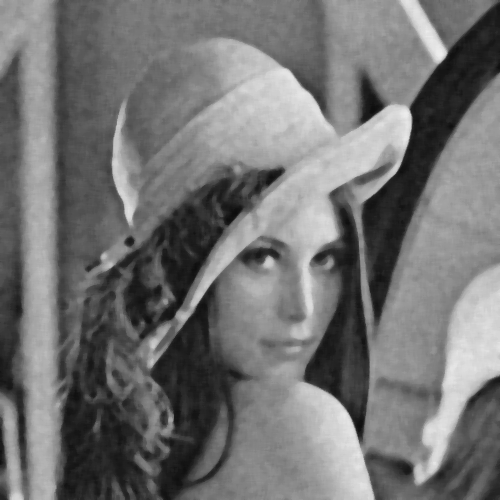
\includegraphics[width=\linewidth]{figs/task1/median_filtered.png}
        \caption{Median Filtered}
    \end{minipage}
    \quad
    \begin{minipage}{0.3\textwidth}
        \centering
        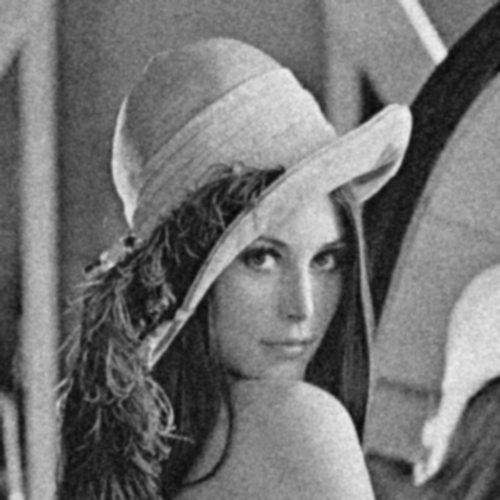
\includegraphics[width=\linewidth]{figs/task1/gaussian_filtered.png}
        \caption{Gaussian Filtered}
    \end{minipage}
\end{figure}

\newpage
\section{Task 2 -- Edge Detection}

\begin{lstlisting}[language=iPython, title=Python Code for Edge Detection]
    import cv2
    import numpy as np
    
    # Read image
    img = cv2.imread("./lenna.png")
    
    # Convert to gray
    gray = cv2.cvtColor(img, cv2.COLOR_BGR2GRAY)
    
    # Define kernels
    sobel_x = np.array([[-1, 0, 1], [-2, 0, 2], [-1, 0, 1]])
    sobel_y = np.array([[-1, -2, -1], [0, 0, 0], [1, 2, 1]])
    
    prewitt_x = np.array([[-1, 0, 1], [-1, 0, 1], [-1, 0, 1]])
    prewitt_y = np.array([[-1, -1, -1], [0, 0, 0], [1, 1, 1]])
    
    # Apply filters
    sobel_x_filtered = cv2.filter2D(gray, -1, sobel_x)
    sobel_y_filtered = cv2.filter2D(gray, -1, sobel_y)
    
    prewitt_x_filtered = cv2.filter2D(gray, -1, prewitt_x)
    prewitt_y_filtered = cv2.filter2D(gray, -1, prewitt_y)
    
    # Save images
    cv2.imwrite("report/figs/task2/sobel_x_filtered.png",
                sobel_x_filtered)
    cv2.imwrite("report/figs/task2/sobel_y_filtered.png",
                sobel_y_filtered)
    cv2.imwrite("report/figs/task2/prewitt_x_filtered.png",
                prewitt_x_filtered)
    cv2.imwrite("report/figs/task2/prewitt_y_filtered.png",
                prewitt_y_filtered)
    
    # Show images
    cv2.imshow("Original", img)
    cv2.imshow("Sobel X Filtered", sobel_x_filtered)
    cv2.imshow("Sobel Y Filtered", sobel_y_filtered)
    cv2.imshow("Prewitt X Filtered", prewitt_x_filtered)
    cv2.imshow("Prewitt Y Filtered", prewitt_y_filtered)
    cv2.waitKey(0)
    cv2.destroyAllWindows()
\end{lstlisting}

\subsection*{Author Contributions \& Comments}
\begin{itemize}[itemsep=-1ex, topsep=0pt, leftmargin=1em]
    \color{RoyalBlue}\item \textbf{Author 1:} \color{black}{--} Devised a pseudo-code for the filtering techniques.
          \color{RoyalBlue}\item \textbf{Author 2:} \color{black}{--} Implemented the Prewwit kernel functions and the Prewitt filtering.
          \color{RoyalBlue}\item \textbf{Author 3:} \color{black}{--} Implemented the Sobel kernel functions and the Sobel filtering.
    \item \textbf{Comments:} From the figures below, we observe that Sobel filter results in more accurate edges than the Prewitt filter. This is attributed to the fact that the Sobel filter gives more weight to the pixels closer to the center of the mask, making it more sensitive to edges, however, this also makes it more sensitive to noise. On the other hand, the Prewitt filter gives equal weight to all pixels in the mask, making it less sensitive to noise, but also less sensitive to edges.
\end{itemize}

\subsubsection*{Results}
\begin{figure}[ht!]
    \centering
    \begin{minipage}{0.3\textwidth}
        \centering
        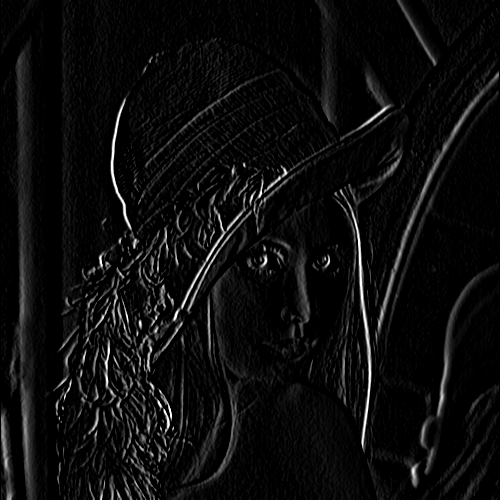
\includegraphics[width=\linewidth]{figs/task2/prewitt_x_filtered.png}
        \caption{Prewitt X Filtered}
    \end{minipage}
    \quad
    \begin{minipage}{0.3\textwidth}
        \centering
        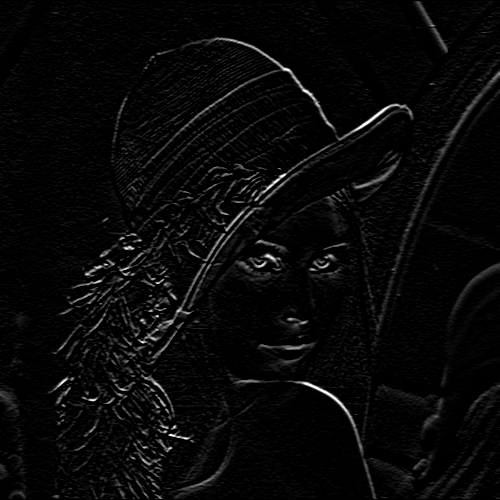
\includegraphics[width=\linewidth]{figs/task2/prewitt_y_filtered.png}
        \caption{Prewitt Y Filtered}
    \end{minipage}
    \vskip 4pt
    \begin{minipage}{0.3\textwidth}
        \centering
        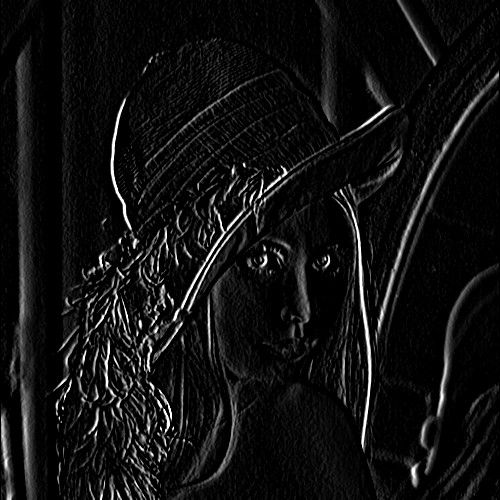
\includegraphics[width=\linewidth]{figs/task2/sobel_x_filtered.png}
        \caption{Sobel X Filtered}
    \end{minipage}
    \quad
    \begin{minipage}{0.3\textwidth}
        \centering
        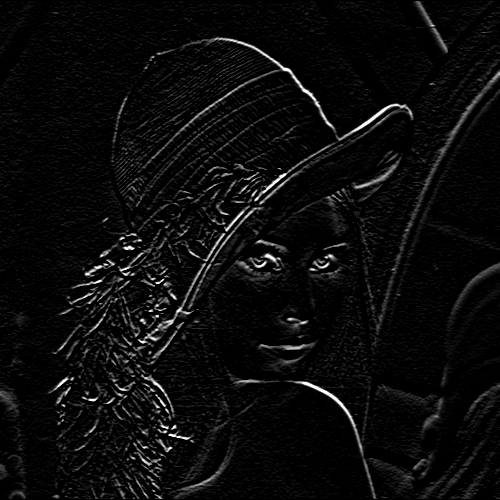
\includegraphics[width=\linewidth]{figs/task2/sobel_y_filtered.png}
        \caption{Sobel Y Filtered}
    \end{minipage}
\end{figure}

\newpage
\section{Task 3 -- Histogram Representation}

\begin{lstlisting}[language=iPython, title=Python Code for Histogram Representation]
    import cv2
    import matplotlib.pyplot as plt
    import numpy as np
    
    def compute_histogram(img):
        gray = cv2.cvtColor(img, cv2.COLOR_BGR2GRAY)
        rows, cols = gray.shape
    
        hist = np.zeros(256)
    
        # Iterate over image and increment histogram
        for i in range(rows):
            for j in range(cols):
                hist[gray[i, j]] += 1
    
        return hist
    
    plt.rcParams["mathtext.fontset"] = "stix"
    plt.rcParams["font.family"] = "STIXGeneral"
    
    # Read image
    img = cv2.imread("./lenna.png")
    
    # Compute histogram
    hist = compute_histogram(img)
    
    # Plot and histogram
    plt.figure(figsize=(16, 6))
    bars = plt.bar(np.arange(256), hist, color="red", edgecolor="black")
    plt.xlabel("Pixel Intensity", fontsize=20)
    plt.ylabel("Frequency", fontsize=20)
    plt.xticks(fontsize=20)
    plt.yticks(fontsize=20)
    plt.xlim(0, 256)
    plt.grid(alpha=0.5)
    plt.legend([bars], ["Pixel Intensity"], fontsize=20)
    plt.tight_layout()
    plt.savefig("report/figs/task3/histogram.png", dpi=300)
    plt.show()
\end{lstlisting}

\subsection*{Author Contributions \& Comments}
\begin{itemize}[itemsep=-1ex, topsep=0pt, leftmargin=1em]
    \color{RoyalBlue}\item \textbf{Author 1:} \color{black}{--} Implemented the iterative histogram computation function.
          \color{RoyalBlue}\item \textbf{Author 2:} \color{black}{--} Made the layout for the histogram plot.
          \color{RoyalBlue}\item \textbf{Author 3:} \color{black}{--} Devised a pseudo-code for the histogram computation function.
    \item \textbf{Comments:} To compute the histogram, we initialize an array of size equal to the number of possible pixel intensities (bit-depth of the image). Then, after converting the image to grayscale, we iterate over each pixel of the image and increment the corresponding index of the histogram array. Finally, we visualize the histogram using a bar graph.
\end{itemize}

\subsubsection*{Results}
\begin{figure}[ht!]
    \centering
    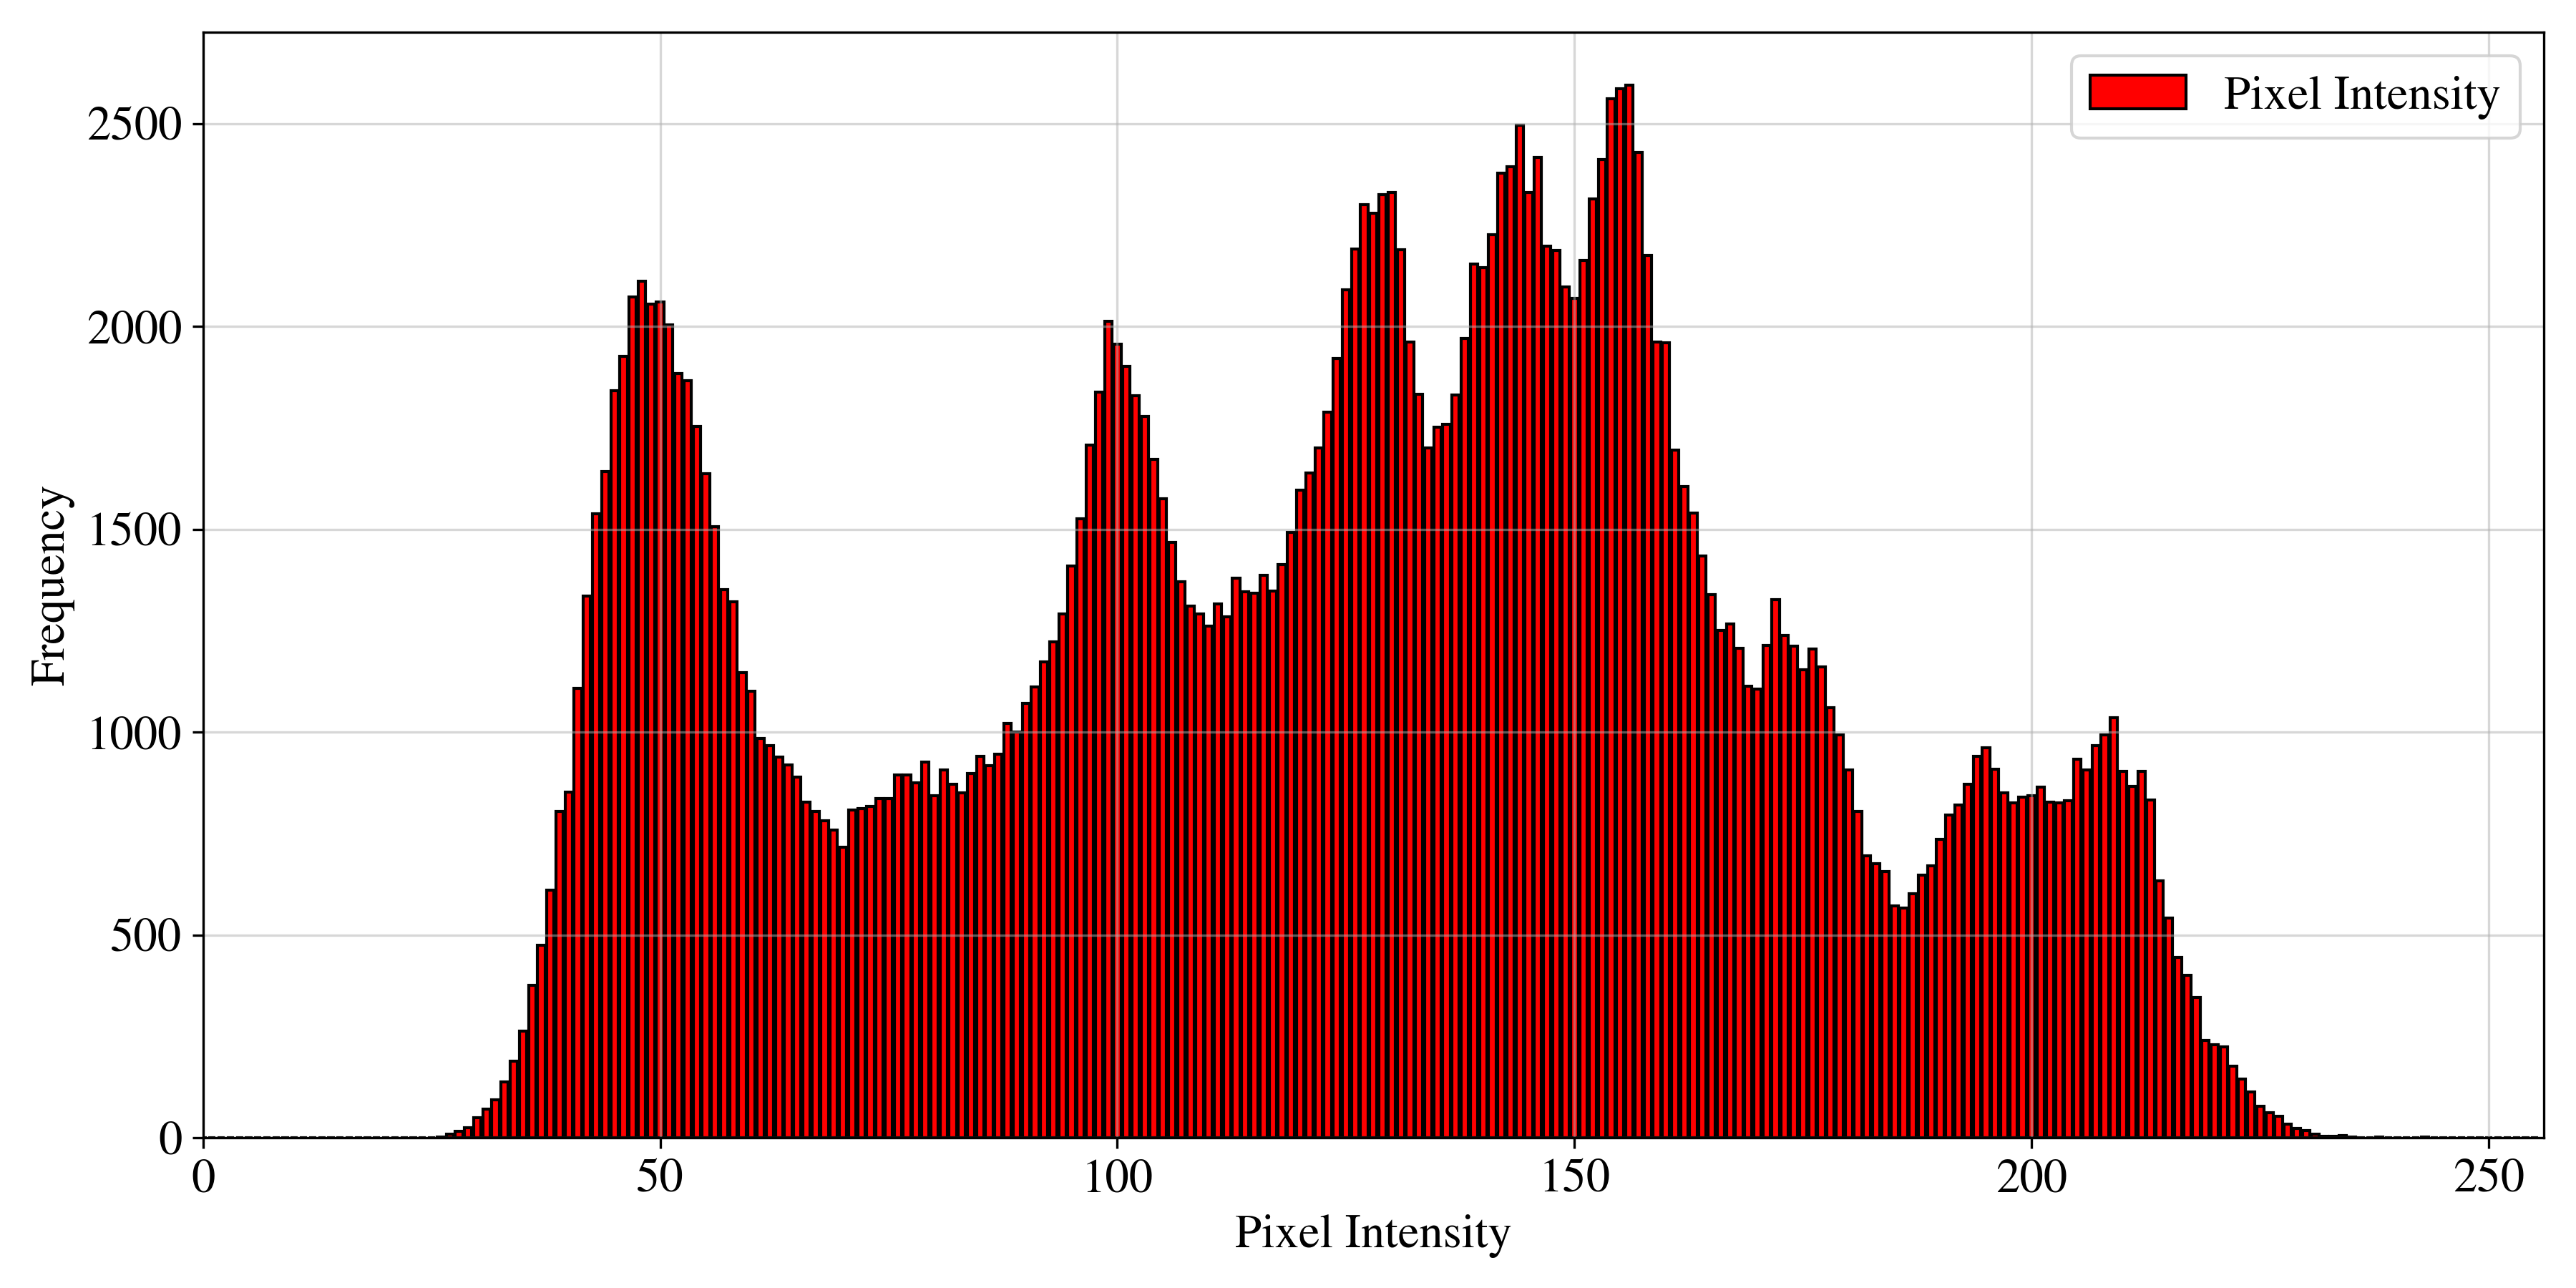
\includegraphics[width=0.85\textwidth]{figs/task3/histogram.png}
    \caption{Histogram Representation}
\end{figure}

\newpage
\section{Task 4 -- Gray and Binary Representation}

\begin{lstlisting}[language=iPython, title=Python Code for Gray and Binary Representation]
    import cv2

    def rgb2gray(rgb):
        """Convert RGB image to grayscale
    
        Standard formula for converting RGB to grayscale
        Reference:
        https://w.wiki/7pNM
        """
    
        # Get the red, green, and blue channels of the image
        red_channel = rgb[:, :, 0]
        green_channel = rgb[:, :, 1]
        blue_channel = rgb[:, :, 2]
    
        # Calculate the grayscale value for each pixel using the 
        # standard formula
        gray = (0.2989 * red_channel + 0.5870 * green_channel + 
                0.1140 * blue_channel)
    
        return gray
    
    # Read image
    img = cv2.imread("./lenna.png")
    
    # Convert to gray
    gray = rgb2gray(img)  # divide by 255 to normalize
    norm_gray = gray / 255
    
    # Convert to binary
    threshold = 127  # empirically found
    binary = gray.copy()
    binary[binary < threshold] = 0
    binary[binary >= threshold] = 255
    
    # Save images
    cv2.imwrite("report/figs/task4/gray.png", gray)
    cv2.imwrite("report/figs/task4/binary.png", binary)
    
    # Show images
    cv2.imshow("Original", img)
    cv2.imshow("Gray", norm_gray)
    cv2.imshow("Binary", binary)
    cv2.waitKey(0)
    cv2.destroyAllWindows()
\end{lstlisting}

\subsection*{Author Contributions \& Comments}
\begin{itemize}[itemsep=-1ex, topsep=0pt, leftmargin=1em]
    \color{RoyalBlue}\item \textbf{Author 1:} \color{black}{--} Implemented the RGB to grayscale conversion function.
          \color{RoyalBlue}\item \textbf{Author 2:} \color{black}{--} Implemented the grayscale to binary conversion function.
          \color{RoyalBlue}\item \textbf{Author 3:} \color{black}{--} Suggested the usage of the standard formula for RGB to grayscale conversion rather than using the OpenCV function.
    \item \textbf{Comments:} To convert an RGB image to grayscale, we utilize the standard formula (\href{https://en.wikipedia.org/wiki/#Converting_color_to_grayscale}{Converting color to grayscale}). To convert a grayscale image to binary, we first empirically find a threshold value, or use a standard value of 127, and then set all pixels below the threshold to 0 and all pixels above the threshold to 255.
\end{itemize}

\subsubsection*{Results}
\begin{figure}[ht!]
    \centering
    \begin{minipage}{0.3\textwidth}
        \centering
        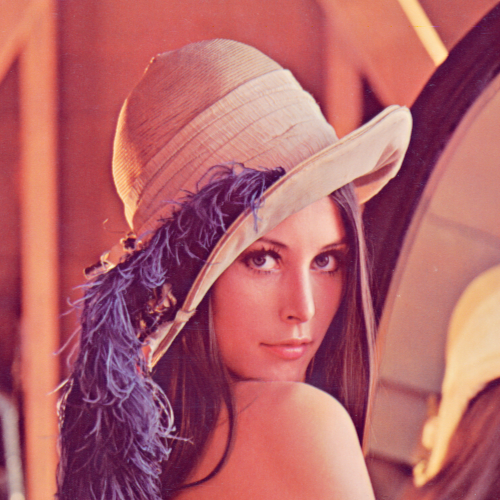
\includegraphics[width=\linewidth]{figs/lenna.png}
        \caption{Original}
    \end{minipage}
    \quad
    \begin{minipage}{0.3\textwidth}
        \centering
        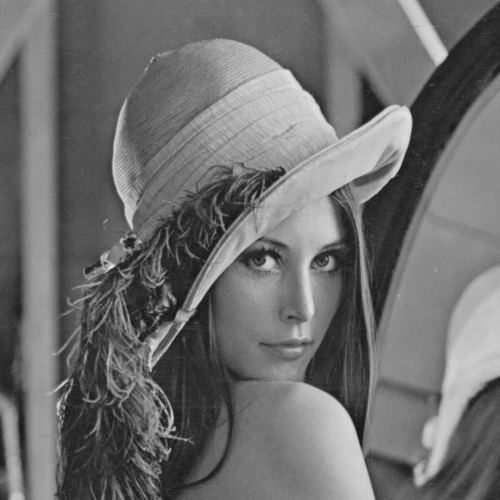
\includegraphics[width=\linewidth]{figs/task4/gray.png}
        \caption{Gray}
    \end{minipage}
    \quad
    \begin{minipage}{0.3\textwidth}
        \centering
        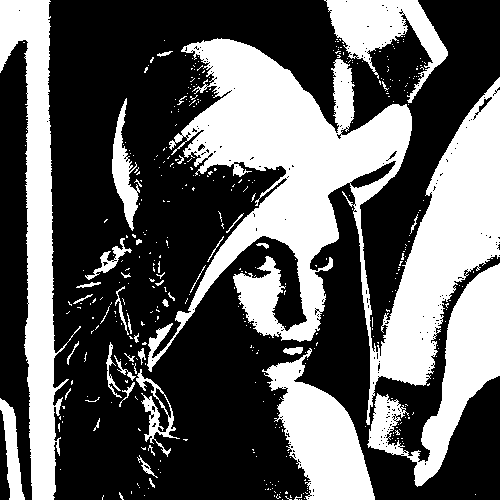
\includegraphics[width=\linewidth]{figs/task4/binary.png}
        \caption{Binary}
    \end{minipage}
\end{figure}

\newpage
\section{Task 5 -- Corner Detection}
\begin{lstlisting}[language=iPython, title=Python Code for Corner Detection]
    import cv2
    import matplotlib.pyplot as plt
    import numpy as np
    from numba import jit
    
    def get_gaussian_kernel(size, sigma=-1):
        """
        Generates a Gaussian kernel of the specified size and sigma.
    
        If sigma = -1, then sigma is automatically calculated
        as (size - 1) / 6.0, as per the OpenCV documentation.
        """
        if sigma < 0:
            sigma = (size - 1) / 6.0
    
        # Generate a grid using the specified size
        axis = np.linspace(-(size - 1) / 2.0, (size - 1) / 2.0, size)
        x, y = np.meshgrid(axis, axis)
    
        # Create the kernel
        gaussian_kernel = np.exp(-0.5 * (x**2 + y**2) / sigma**2)
    
        return gaussian_kernel / np.sum(gaussian_kernel)
    
    # Details of JIT in comments
    @jit(nopython=True)
    def non_max_suppression(H_response, win_height, win_width):
        """
        Performs non-maximum suppression on the Harris response.
        """
        for i in range(win_height, H_response.shape[0] - win_height):
            for j in range(win_width, H_response.shape[1] - win_width):
                if H_response[i, j] == 0:
                    continue
                H_slice = H_response[i - win_height : i + win_height + 1,
                                     j - win_width : j + win_width + 1]
                if H_response[i, j] != H_slice.max():
                    H_response[i, j] = 0
        return H_response

    @jit(nopython=True)
    def get_harris_matrix(I_x, I_y, w, i, j, win_height, win_width):
        """
        Returns the Harris matrix for the pixel at (i, j).
        """
        I_x_slice = I_x[i - win_height : i + win_height + 1,
        j - win_width : j + win_width + 1]
        I_y_slice = I_y[i - win_height : i + win_height + 1,
                        j - win_width : j + win_width + 1]
        M_xx = np.sum(I_x_slice**2 * w)
        M_yy = np.sum(I_y_slice**2 * w)
        M_xy = np.sum(I_x_slice * I_y_slice * w)
        return np.array([[M_xx, M_xy], [M_xy, M_yy]])
    
    @jit(nopython=True)
    def get_cornerness(M, k):
        """
        Returns the cornerness of the Harris matrix.
        """
        return np.linalg.det(M) - k * np.trace(M) ** 2
    
    # Read image
    img = cv2.imread("./task5.png")
    
    # Convert to gray
    gray = cv2.cvtColor(img, cv2.COLOR_BGR2GRAY)
    gray = gray.astype(np.float32) / gray.max()
    
    # Compute Ix and Iy
    sobel_x = np.array([[-1, 0, 1], [-2, 0, 2], [-1, 0, 1]])
    sobel_y = np.array([[-1, -2, -1], [0, 0, 0], [1, 2, 1]])
    
    I_x = cv2.filter2D(gray, -1, sobel_x)
    I_y = cv2.filter2D(gray, -1, sobel_y)
    
    # Harris corner detection
    kernel_size = 9
    window_shape = (kernel_size, kernel_size)
    win_height, win_width = ((window_shape[0] - 1) // 2,
                             (window_shape[1] - 1) // 2)
    w = get_gaussian_kernel(kernel_size)

    H_response = np.zeros(gray.shape, dtype=np.float32)
    k = 0.04
    
    for i in range(win_height, gray.shape[0] - win_height):
        for j in range(win_width, gray.shape[1] - win_width):
            M = get_harris_matrix(I_x, I_y, w, i, j,
                                  win_height, win_width)
            H_response[i, j] = get_cornerness(M, k)
    
    # Thresholding
    # Empirically found values
    threshold = 0.05 * H_response.max()
    H_response[H_response < threshold] = 0
    
    # Non-maximum suppression
    H_response = non_max_suppression(H_response, win_height, win_width)
    
    # Get corners
    y_c, x_c = np.nonzero(H_response)
    
    # Draw circles on the image
    for i in range(len(x_c)):
        cv2.circle(img, (x_c[i], y_c[i]), 5, (0, 0, 255), -1)
    
    # Save the image
    cv2.imwrite("report/figs/task5/corners.png", img)
    
    # Display the image with circles
    cv2.imshow("Corners", img)
    cv2.waitKey(0)
    cv2.destroyAllWindows()
\end{lstlisting}

\subsection*{Author Contributions \& Comments}
\begin{itemize}[itemsep=-1ex, topsep=0pt, leftmargin=1em]
    \color{RoyalBlue}\item \textbf{Author 1:} \color{black}{--} Implemented functions for computing the Harris response matrix and the cornerness measure. Also proposed the usage of JIT compilation to optimize the code.
          \color{RoyalBlue}\item \textbf{Author 2:} \color{black}{--} Implemented the Gaussian kernel function and the non-maximum suppression function. Also implemented the placement of circles on the image.
          \color{RoyalBlue}\item \textbf{Author 3:} \color{black}{--} Patched the code together and realized the corner detection algorithm with thresholding.
    \item \textbf{Comments:} To perform Harris corner detection, we first compute the image gradients $I_x$ and $I_y$ using the Sobel operator. Then, we compute the Harris matrix for each pixel in the image, and use it to compute the cornerness of the pixel. Finally, we threshold the cornerness values and perform non-maximum suppression to obtain the corners.\\Additionally, to optimize the code, we use the \lstinline{numba} library to Just-In-Time (JIT) compile the functions to boost the execution time incurred by the \lstinline{for} loops. The JIT compilation is done by adding the \lstinline{@jit(nopython=True)} decorator above the function definition.
\end{itemize}

\subsubsection*{Results}
\begin{figure}[ht!]
    \centering
    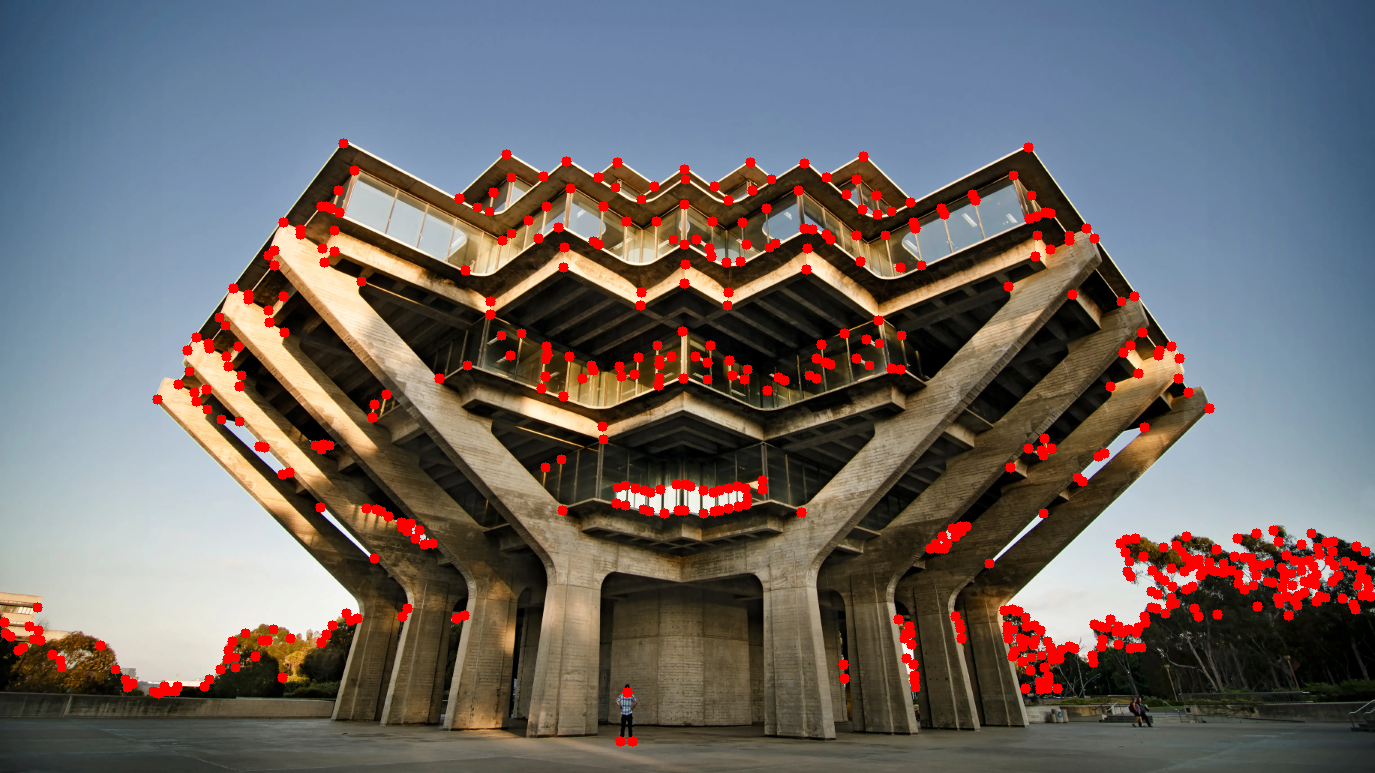
\includegraphics[width=0.85\textwidth]{figs/task5/corners.png}
    \caption{Detected Corners}
\end{figure}

\end{document}